\nextslide{1. Basic principles}
\begin{enumerate}
\item Some basics
\item Jack
\item ESC/Java
\end{enumerate}

\nextslide{Some basics}
\small
The {\purple Java Modelling Language} (JML)
is used to annotate the Java programs we want to verify with 
Jack or ESC/Java.\\
Jack and ESC/Java use a {\purple weakest precondition calculus} to generate
the proof obligations.\\
In JML you can express loop invariants, assertions method's
pre and post conditions.\\
JML has a really large syntax so every tool (except maybe JMLrac)
implements only a {\purple portion} of its syntax.


\nextslide{Jack}
\small
\blist
\item Programmed mainly by Lilian Burdy
\item At first single prover (B)
\item Multi-prover interface (Simplify, Coq, PVS)
\item Fully integrated in {\purple Eclipse} as a plugin, and use a 
{\purple plugin architecture} to include new provers
\elist
\begin{center}
\includegraphics[width= \linewidth]{jack.ps}
\end{center}
\nextslide{ESC/Java} 
\small
\blist
\item Joe Kiniry et al.
\item At first single prover (Simplify)
\item Now beginning to be multi-prover   (PVS, Coq...)\\
  \rarrow the work of Cl\'ement Hurlin and Carl Pulley\\
and wishing to be fully integrated in eclipse!
\elist
\begin{center}
  \includegraphics[width= 0.86\linewidth]{escjava.ps}
\end{center}

